% =====================================================================
%  Introduction to Deep Learning — Class 26
%  Topic (course plan): Recurrent Neural Network
%  Subtopic (course plan): Back-prop over time and Bidirectional RNNs
%  Sources (course plan): Jurafsky & Martin Ch. 13 (Ch. 14 in the
%    August 2026 draft), Goodfellow Ch. 10
%
%  The first lecture of the RNN block: the recurrent network as a
%  dynamical system unfolded into a computational graph with shared
%  parameters; forward inference; back-propagation through time as
%  ordinary back-propagation on the unfolded graph, written out; its
%  cost; truncation; the bidirectional network.  Classes 27-29 assume
%  exactly this.
%
%  Every measured figure is produced by src/ on the tape of Class 27:
%  BPTT written by hand and checked against the tape and finite
%  differences, the per-step terms of the gradient, timings, truncated
%  training on a recall task, and the influence maps of a one- and a
%  two-directional network.  C variant: the B deck with the one result
%  stated in neither textbook (what truncation removes) replaced by the
%  book's own words.  See _shared/PLAN_Classes26_27_28_29.md.
%
%  Compile:  xelatex main.tex   (run twice)
% =====================================================================
\documentclass[aspectratio=169, 11pt]{beamer}

\usetheme{metropoliscustom}

\usepackage{graphicx}
\DeclareGraphicsExtensions{.pdf,.png,.jpg}
\graphicspath{{figs/}{Class26_BPTT_Bidirectional_RNNs/C_Textbook_Theorems_Only/figs/}}
\usepackage{amsmath, amssymb}
\usepackage{bm}
\usepackage{tikz}
\usetikzlibrary{arrows.meta, positioning, calc, decorations.pathreplacing,
                shapes.geometric, fit, backgrounds}
\tcbuselibrary{skins}

\definecolor{shc}{HTML}{341651}
\definecolor{tealc}{HTML}{1C7293}
\definecolor{dpc}{HTML}{800000}
\definecolor{accc}{HTML}{B8860B}

% ---- theorem environments -------------------------------------------
\setbeamertemplate{theorems}[numbered]
\usepackage{remreset}
\makeatletter\@removefromreset{theorem}{section}\makeatother
\renewcommand{\thetheorem}{\arabic{theorem}}
\newtheorem{lemmax}[theorem]{Lemma}
\newtheorem{propx}[theorem]{Proposition}
\newtheorem{corx}[theorem]{Corollary}
\newtheorem{defx}[theorem]{Definition}
\newtheorem{thmx}[theorem]{Theorem}

\newcommand{\bridge}[1]{%
  {\scriptsize\itshape\color{mcMuted} #1\par}\vspace{0.35em}}

\newcommand{\srcline}[1]{%
  \par\vspace{0.25em}%
  {\scriptsize\color{mcMuted}\hfill #1\par}}

\newcommand{\figsource}[1]{{\scriptsize\color{mcMuted} #1}}
\newcommand{\figcap}[2][0.90]{%
  \begin{center}\begin{minipage}{#1\textwidth}\centering
    {\scriptsize\color{mcMuted} #2}
  \end{minipage}\end{center}}

% =====================================================================
\title{Recurrent Neural Networks}
\subtitle{Back-propagation Through Time and Bidirectional RNNs}
\author{Introduction to Deep Learning \ \textperiodcentered\ Class 26}
\institute{}
\date{}

\footleft{Introduction to Deep Learning}
\footright{BPTT and Bidirectional RNNs}
\titlelogos{}

\begin{document}

\maketitle

\begin{frame}{Outline}
  \tableofcontents
\end{frame}

% =====================================================================
\section{From Space to Time}
% =====================================================================

\begin{frame}{Where we are coming from}
  \vspace{-0.3em}
  {\scriptsize
  \renewcommand{\arraystretch}{1.3}
  \begin{tabular}{@{}l@{\hspace{1.2em}}l@{}}
    \textbf{Classes 23--25: convolution} & \textbf{what it gave us}\\
    the input is a \alert{grid} of fixed size --- an image & one kernel slides over every position\\
    nearby pixels matter most & locality: each output sees a small window\\
    a cat is a cat wherever it sits & equivariance: the same weights everywhere\\
    a kernel has few weights, an image many pixels & parameter sharing across \alert{space}\\
  \end{tabular}}
  \vspace{0.4em}

  {\footnotesize
  \begin{itemize}\itemsep0.2em
    \item All of it rests on the input being a fixed-size grid in which
          position is \alert{where}
    \item Today's data is an \alert{ordered list of variable length},
          position is \alert{when}, and what matters may be far back
    \item The instinct carries over --- one set of weights, reused
          everywhere --- but ``everywhere'' will mean every \alert{time
          step}, plus one new wire
  \end{itemize}}
  \srcline{Classes 23--25; Goodfellow et al.\ (2016), \S10 opening; Jurafsky \& Martin (2026), Ch.~14 opening.}
\end{frame}

\begin{frame}{The data: sequences}
  \vspace{0.05em}
  {\footnotesize
  \begin{itemize}\itemsep0.25em
    \item A \alert{sequence} is an ordered list $\mathbf{x}_1, \ldots, \mathbf{x}_\tau$
          whose length $\tau$ varies: the words of a sentence, the frames
          of a recording, the readings of a sensor
    \item \alert{Order matters}: ``dog bites man'' and ``man bites dog''
          have the same words; a bag of features loses the point
    \item \alert{Length varies}: a five-word and a fifty-word sentence
          are both sentences; a fixed input size cannot take both
    \item \alert{Dependencies reach}: the word that decides the next may
          be six words back, or sixty --- language is ``an inherently
          temporal phenomenon''
  \end{itemize}}
  \vspace{0.1em}
  \begin{redhighlight}
    A sequence model must take any length, respect the order, and let
    the distant past reach the present. No tool so far does all three.
  \end{redhighlight}
  \srcline{Jurafsky \& Martin (2026), Ch.~14 opening; Goodfellow et al.\ (2016), \S10 opening.}
\end{frame}

\begin{frame}{What natural language processing asks of a model}
  \vspace{-0.4em}
  \begin{center}
    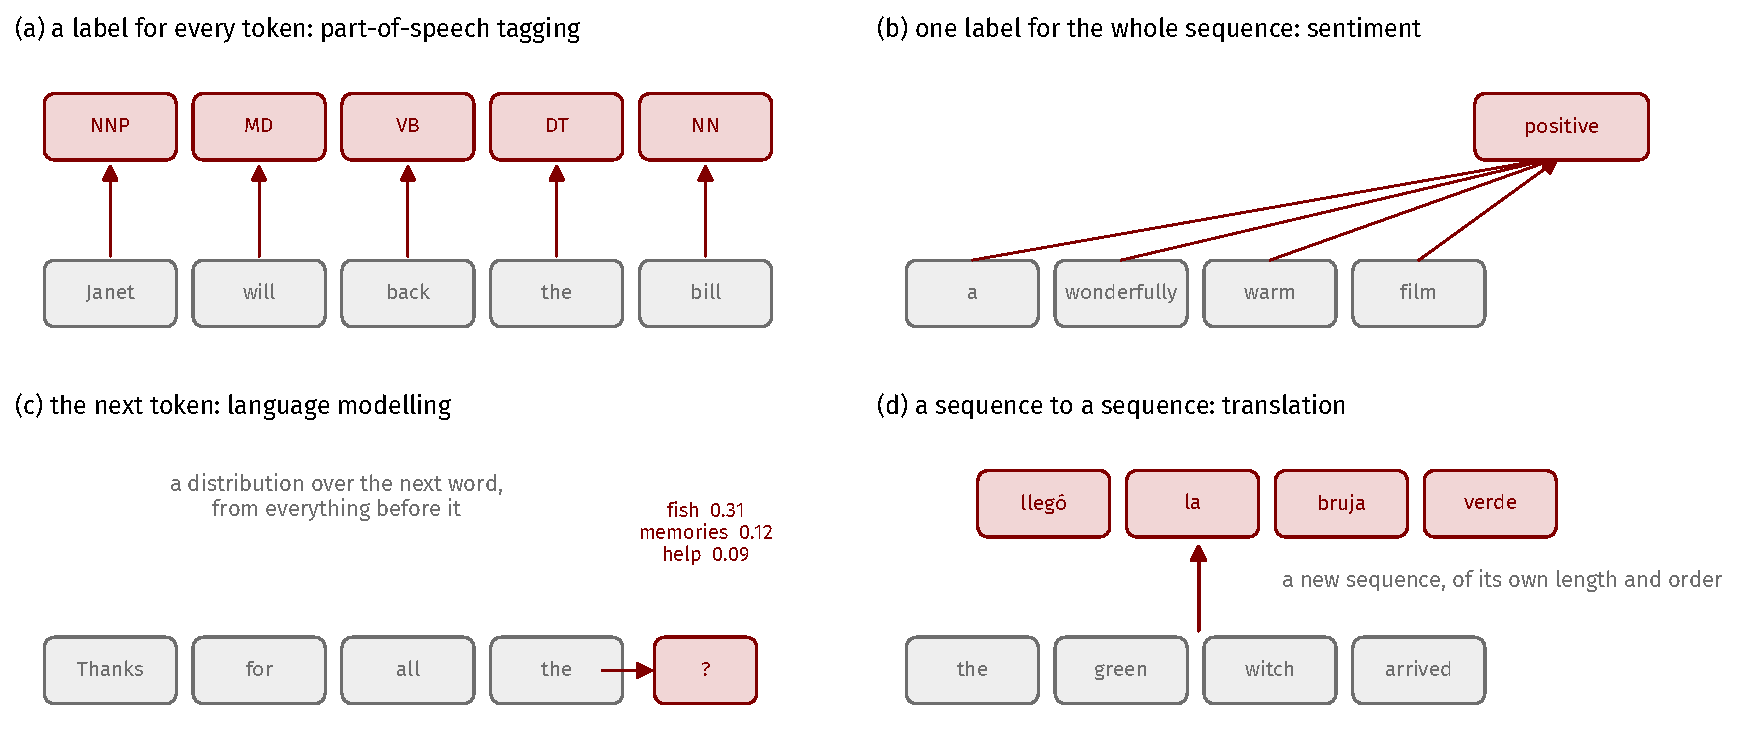
\includegraphics[width=0.88\linewidth]{sequence_tasks}
  \end{center}
  \vspace{-0.6em}
  {\tiny\color{mcMuted}
  Four shapes of problem, all with a sequence in: (a) a label for every
  token, as in part-of-speech tagging or named-entity recognition; (b)
  one label for the whole sequence, as in sentiment analysis or spam
  detection; (c) the next token given the previous ones --- a language
  model, which is what a chat model or a keyboard suggestion is; (d) a
  whole new sequence, of its own length, as in translation, summarisation
  or speech recognition.
  \hfill Jurafsky \& Martin (2026), \S14.2--14.3, \S14.6, Fig.~14.15.\par}
\end{frame}

\begin{frame}{NLP, in one paragraph}
  \vspace{0.05em}
  {\footnotesize
  \begin{itemize}\itemsep0.25em
    \item \alert{Natural language processing}: getting a machine to
          read, understand and produce human language --- text, and
          speech turned into text
    \item Its raw material is a sequence of discrete symbols --- words,
          characters, sub-word pieces --- each turned into a vector, an
          \alert{embedding}: a one-hot input times a matrix
    \item Its fundamental move is to \alert{predict}: the next word, the
          tag of this word, the sentiment of this review, the translation
          of this sentence
    \item Its difficulty is \alert{context}: a word's meaning is fixed by
          words anywhere in the sentence --- before it, or after it
  \end{itemize}}
  \vspace{0.1em}
  \begin{redhighlight}
    The recurrent network is the first architecture built to read a
    sequence of any length, one token at a time, keeping what it has read.
  \end{redhighlight}
  \srcline{Jurafsky \& Martin (2026), Ch.~14 opening, \S14.2, \S14.3.}
\end{frame}

\begin{frame}{Why the tools we have fall short}
  \vspace{-0.4em}
  \begin{center}
    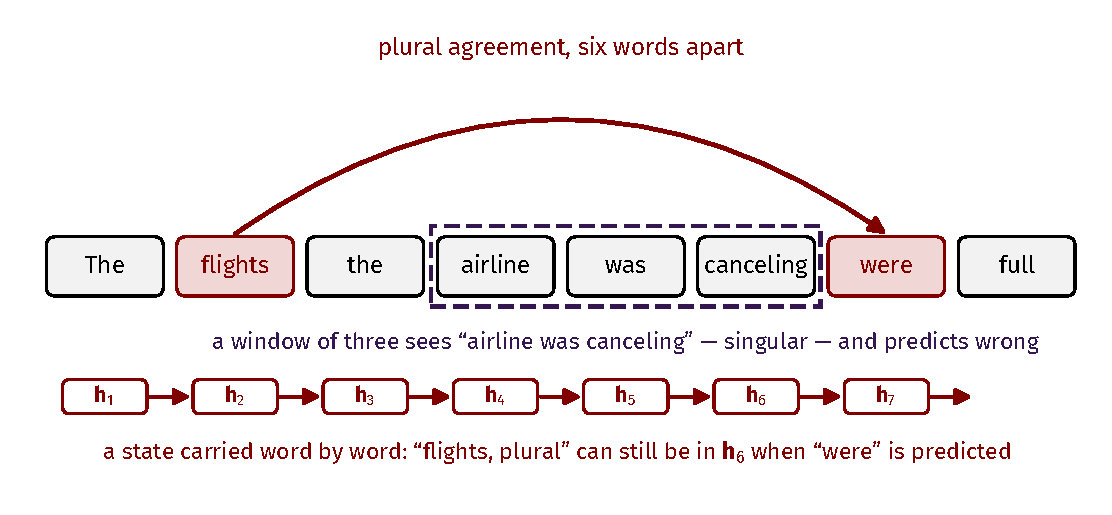
\includegraphics[width=0.78\linewidth]{window_fails}
  \end{center}
  \vspace{-0.6em}
  {\tiny\color{mcMuted}
  Jurafsky \& Martin's sentence: the verb \emph{were} must agree with
  \emph{flights}, six words back, and the nearer noun \emph{airline} is
  singular. A feedforward network on a window of $k$ words --- and a
  one-dimensional convolution, which is the same window slid along ---
  sees only \emph{airline was canceling} and cannot get this right for
  any $k$ smaller than the gap; and the gap has no bound, so no $k$ is
  big enough. A state carried word by word can.
  \hfill Jurafsky \& Martin (2026), \S14.2, \S14.5, example (14.19).\par}
\end{frame}

\begin{frame}{The idea: from sharing across space to sharing across time}
  \vspace{-0.4em}
  \begin{center}
    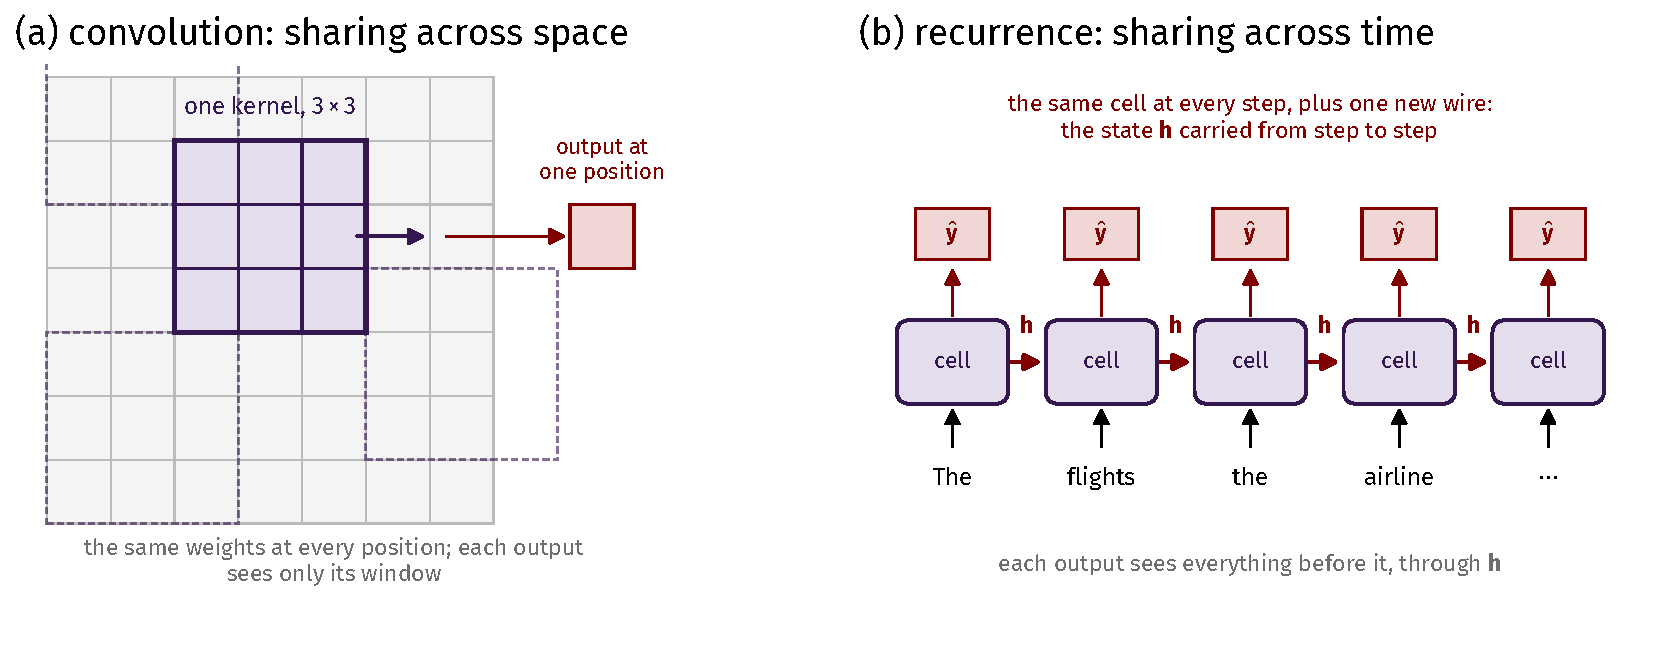
\includegraphics[width=0.74\linewidth]{space_vs_time}
  \end{center}
  \vspace{-0.6em}
  {\tiny\color{mcMuted}
  (a) A convolution applies the same kernel at every position of the
  grid; each output depends only on its window. (b) A recurrent network
  applies the same cell at every step of the sequence, and adds one wire:
  the state $\mathbf{h}$, passed from each step to the next, so that each
  output depends on everything before it. The parallel is exact: sharing
  across space gave equivariance and few parameters; sharing across time
  gives a model of any length with few parameters, and the new wire buys
  memory.
  \hfill Goodfellow et al.\ (2016), \S10 opening, \S10.1; Class 23.\par}
\end{frame}

\begin{frame}{How the recurrent network reads the sentence}
  \vspace{-0.4em}
  \begin{center}
    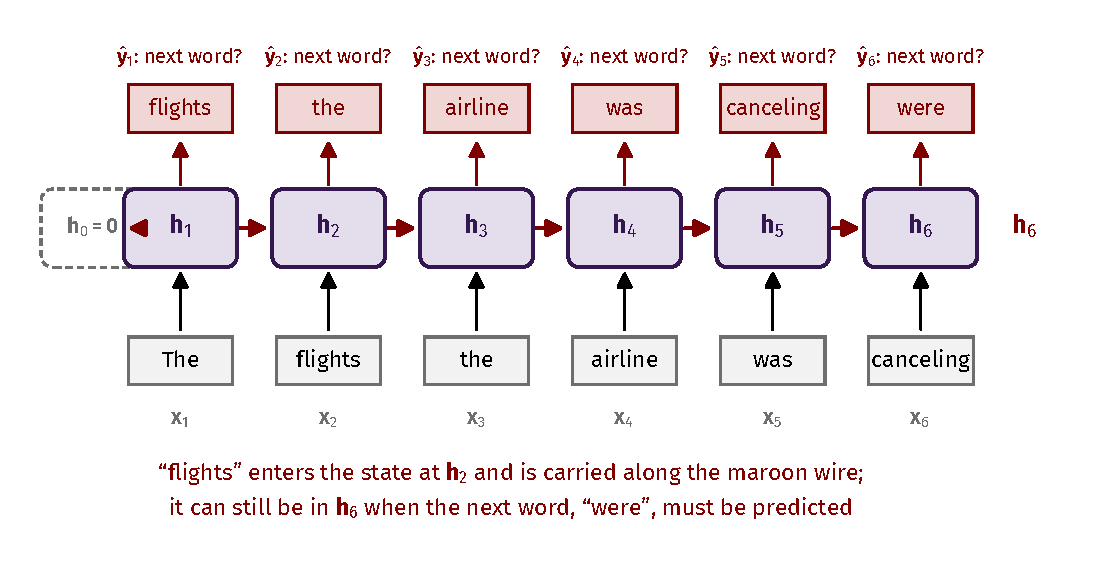
\includegraphics[width=0.72\linewidth]{running_example}
  \end{center}
  \vspace{-0.6em}
  {\tiny\color{mcMuted}
  The running example, read one word at a time. At each step the cell
  takes the current word $\mathbf{x}_t$ and the state $\mathbf{h}_{t-1}$,
  produces a new state $\mathbf{h}_t$ --- a summary of everything read so
  far --- and from it a prediction $\hat{\mathbf{y}}_t$ of the next word.
  \emph{flights} enters the state at $t = 2$ and, if the network has
  learned to keep it, is still there at $t = 6$ when \emph{were} is due.
  The state has a fixed size whatever the length of the sentence: a lossy
  summary, and training decides what it keeps.
  \hfill Jurafsky \& Martin (2026), \S14.1--14.2; Goodfellow et al.\ (2016), \S10.1.\par}
\end{frame}

\begin{frame}{The block ahead, and where today sits}
  \vspace{0.1em}
  {\scriptsize
  \renewcommand{\arraystretch}{1.3}
  \begin{tabular}{@{}l@{\hspace{0.8em}}l@{\hspace{0.8em}}l@{}}
    \textbf{Class} & \textbf{the problem} & \textbf{the answer}\\
    \alert{26 --- today} & how is a sequence read, and the reader trained? & the cell, unfolding, BPTT\\
    27 --- encoder--decoder & how is one sequence read and another written? & two chains, a context, attention\\
    28 --- LSTM and gates & why is the far past forgotten; what fixes it? & the gradient across time; gates\\
    29 --- NLP tasks & which output goes with which task? & language models, taggers, classifiers\\
    30--31 --- transformers & can a sequence be read without the chain? & attention without recurrence\\
  \end{tabular}}
  \vspace{0.4em}

  {\footnotesize
  \begin{itemize}\itemsep0.2em
    \item Today builds the machine and trains it; the classes after put
          it to work, open it up, and replace it. Two questions run through
          today: what does one step compute, and how does a loss at the end
          reach a weight used at the start?
  \end{itemize}}
  \srcline{Course plan, Classes 26--31; Jurafsky \& Martin (2026), \S14.6.}
\end{frame}

% =====================================================================
\section{The Recurrent Network}
% =====================================================================

\begin{frame}{A network with a cycle}
  \vspace{-0.2em}
  {\footnotesize
  \begin{itemize}\itemsep0.25em
    \item The picture two slides back has one feature no network of
          this course has had: an edge that goes \alert{back} --- the state
          $\mathbf{h}$ leaves the cell and re-enters it at the next step.
          Any network with such a cycle is a \alert{recurrent neural network}
    \item Cycles in general are hard to reason about and train. Elman's
          \alert{simple recurrent network} has exactly one: the hidden
          layer of step $t-1$ feeds the hidden layer of step $t$
    \item That one edge is the memory: the previous hidden layer is a
          summary of the whole past --- \emph{flights} at $t = 6$ --- with
          no fixed window
    \item The rest is ordinary: input, hidden and output layers, one
          feedforward step per token. So: what exactly does the step
          compute, and how does the cycle change training?
  \end{itemize}}
  \srcline{Jurafsky \& Martin (2026), \S14.1; Goodfellow et al.\ (2016), \S10.1; Elman (1990).}
\end{frame}
\begin{frame}{Notation for today}
  \vspace{-0.3em}
  {\footnotesize
  \renewcommand{\arraystretch}{1.22}
  \begin{tabular}{@{}l@{\hspace{1.4em}}l@{}}
    $\mathbf{x}_t \in \mathbb{R}^{d_{\mathrm{in}}}$ & input at step $t$; $\tau$ or $n$ the sequence length; $\mathbf{h}_0 = \mathbf{0}$\\
    $\mathbf{h}_t \in \mathbb{R}^{d_h}$ & hidden state; $\mathbf{a}_t$ its pre-activation\\
    $\mathbf{W}$, $\mathbf{U}$, $\mathbf{V}$ & input-to-hidden, hidden-to-hidden, hidden-to-output; biases $\mathbf{b}, \mathbf{c}$\\
    $\mathbf{o}_t$, $\hat{\mathbf{y}}_t = \mathrm{softmax}(\mathbf{o}_t)$ & output scores and distribution; $\mathbf{y}_t$ the target, $L_t$ the loss at $t$\\
    $g$, $g'$ & the hidden activation ($\tanh$ throughout) and its derivative, $1 - \mathbf{h}_t^2$\\
    $\nabla_{\mathbf{h}_t}L$ & the gradient of the total loss on the state at $t$\\
    $\mathbf{h}^{f}_t,\ \mathbf{h}^{b}_t$, $[\,\cdot\,;\,\cdot\,]$ & forward and backward states; concatenation; $L = \sum_t L_t$\\
  \end{tabular}}
  \vspace{0.3em}

  \begin{alertblock}{Two conventions, one line}
    \small Jurafsky: $\mathbf{W}$ input, $\mathbf{U}$ recurrence,
    $\mathbf{V}$ output, time as a subscript. Goodfellow swaps
    $\mathbf{U}$ and $\mathbf{W}$ and writes $\mathbf{h}^{(t)}$. This
    block keeps Jurafsky's letters.
  \end{alertblock}
  \srcline{Jurafsky \& Martin (2026), \S14.1.1; Goodfellow et al.\ (2016), \S10.2.}
\end{frame}

\begin{frame}{The simple recurrent network}
  \vspace{-0.45em}
  \begin{defx}[Simple recurrent network]\label{th:rnn}
    \small
    With $\mathbf{h}_0 = \mathbf{0}$, for $t = 1, \ldots, \tau$:
    \[
      \mathbf{a}_t = \mathbf{b} + \mathbf{U}\mathbf{h}_{t-1} + \mathbf{W}\mathbf{x}_t, \qquad
      \mathbf{h}_t = \tanh(\mathbf{a}_t), \qquad
      \mathbf{o}_t = \mathbf{c} + \mathbf{V}\mathbf{h}_t, \qquad
      \hat{\mathbf{y}}_t = \mathrm{softmax}(\mathbf{o}_t).
    \]
    The parameters $\mathbf{U}, \mathbf{W}, \mathbf{V}, \mathbf{b}, \mathbf{c}$ are the same at every step.
  \end{defx}
  \vspace{-0.1em}
  {\footnotesize
  \begin{itemize}\itemsep0.16em
    \item Read it as the picture: the cell at step $t$ takes two things,
          \alert{what it sees now} ($\mathbf{x}_t$) and \alert{what it
          remembers} ($\mathbf{h}_{t-1}$), mixes them, squashes, and hands the
          result on as the new memory $\mathbf{h}_t$
    \item From that memory it makes a prediction, $\hat{\mathbf{y}}_t$: a
          distribution over the next word, or the tag of this word ---
          whatever the task asks for
    \item Forward inference is \alert{incremental}: $\mathbf{h}_t$ needs
          $\mathbf{h}_{t-1}$, so the sequence is read start to end
  \end{itemize}}
  \srcline{Jurafsky \& Martin (2026), Eqs.~14.1--14.3, Figs.~14.1--14.3; Goodfellow et al.\ (2016), Eqs.~10.8--10.11.}
\end{frame}

\begin{frame}{Each term, in words}
  \vspace{-0.1em}
  {\scriptsize
  \renewcommand{\arraystretch}{1.3}
  \begin{tabular}{@{}l@{\hspace{0.9em}}l@{\hspace{0.9em}}l@{}}
    \textbf{term} & \textbf{what it is} & \textbf{in the running sentence, at \emph{airline}}\\
    $\mathbf{x}_t$ & the input at step $t$, an embedding & the vector for \emph{airline}\\
    $\mathbf{W}\mathbf{x}_t$ & how the current input pushes the state & ``a singular noun just came in''\\
    $\mathbf{h}_{t-1}$ & the memory: a summary of $\mathbf{x}_1 \ldots \mathbf{x}_{t-1}$ & ``inside a clause about \emph{flights}''\\
    $\mathbf{U}\mathbf{h}_{t-1}$ & what of the memory is kept, and how it is rearranged & keep \emph{flights}, note the clause\\
    $\mathbf{b}$, $\tanh$ & a bias, and a squash that keeps the state in $(-1, 1)$ & nothing blows up over a long sentence\\
    $\mathbf{h}_t$ & the new memory, passed to step $t+1$ & everything so far, in $d_h$ numbers\\
    $\mathbf{V}\mathbf{h}_t$, softmax & the read-out: a score for every possible output & \emph{was} likely, \emph{were} less --- for now\\
  \end{tabular}}
  \vspace{0.3em}

  {\footnotesize
  \begin{itemize}\itemsep0.15em
    \item Three matrices, three jobs: $\mathbf{W}$ \alert{reads}, $\mathbf{U}$
          \alert{remembers}, $\mathbf{V}$ \alert{answers}; the same three at
          every step, so their sizes do not depend on the sentence
    \item What $\mathbf{U}$ keeps and drops is learned from the loss --- the second half of today
  \end{itemize}}
  \srcline{Jurafsky \& Martin (2026), \S14.1--14.1.1; Goodfellow et al.\ (2016), \S10.1--10.2.}
\end{frame}

\begin{frame}{The simple recurrent network, drawn}
  \begin{center}
    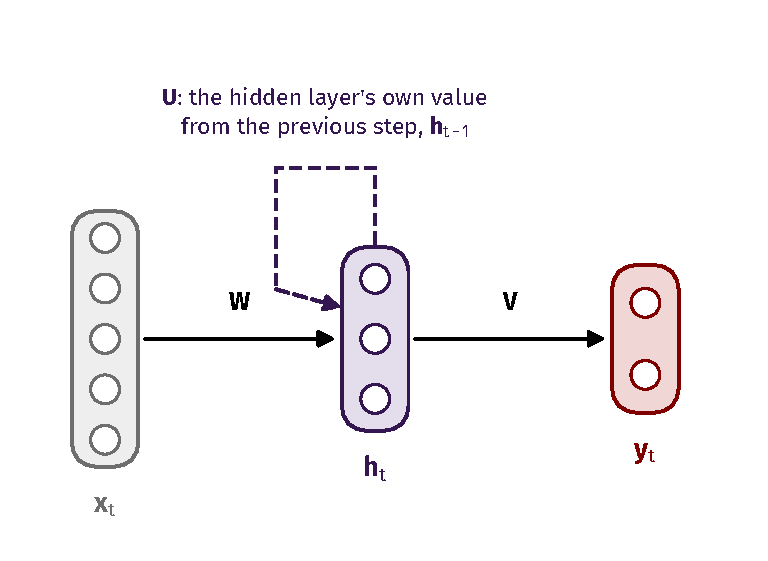
\includegraphics[width=0.52\linewidth]{elman_network}
  \end{center}
  \vspace{-0.5em}
  {\tiny\color{mcMuted}
  The Elman network: an input layer, a hidden layer and an output
  layer, as in every feedforward network of this course, plus one
  recurrent link (dashed): the hidden layer's own activation from the
  previous step is part of its input. $\mathbf{W}$ reads the input,
  $\mathbf{U}$ carries the memory, $\mathbf{V}$ produces the output.
  \hfill Layout of Jurafsky \& Martin (2026), Fig.~14.1.\par}
\end{frame}

\begin{frame}{The same network, as one feedforward step}
  \begin{center}
    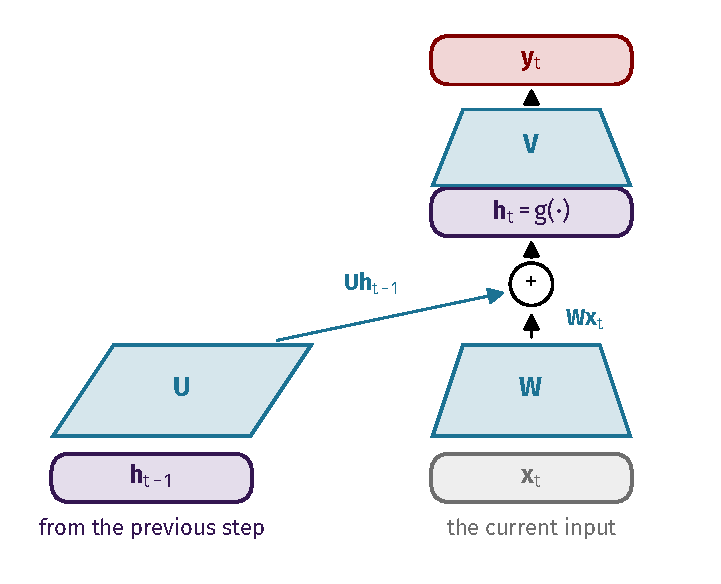
\includegraphics[width=0.44\linewidth]{elman_feedforward}
  \end{center}
  \vspace{-0.5em}
  {\tiny\color{mcMuted}
  The recurrence unpacked: the previous hidden layer $\mathbf{h}_{t-1}$ is
  multiplied by $\mathbf{U}$ and added to the feedforward component
  $\mathbf{W}\mathbf{x}_t$; the sum goes through the activation $g$ to give
  $\mathbf{h}_t$, and $\mathbf{V}$ turns it into $\mathbf{y}_t$. Given
  $\mathbf{h}_{t-1}$, this is the standard calculation of Class 5 with two
  inputs; the only new set of weights is $\mathbf{U}$.
  \hfill Layout of Jurafsky \& Martin (2026), Fig.~14.2.\par}
\end{frame}

\begin{frame}{Why unfold}
  \vspace{0.05em}
  {\footnotesize
  \begin{itemize}\itemsep0.25em
    \item The picture with the cycle is compact but says nothing about
          \alert{how to compute}: a cycle has no first node, and every
          gradient rule of Class 11 was for a graph without cycles
    \item The trick: give every time step its \alert{own copy} of the
          cell. The cycle becomes a chain $\mathbf{h}_0 \to \mathbf{h}_1 \to \cdots \to \mathbf{h}_\tau$,
          a directed acyclic graph as long as the sequence
    \item This buys three things: the forward pass is a walk along the
          chain; back-propagation is Class 11's algorithm on it,
          unchanged; and the parameters, shared by all the copies, are
          still one set, however long the chain
    \item It also puts today's two questions on the page: which
          computations happen, in what order, and along which paths a
          loss at the end reaches a weight used at the start
  \end{itemize}}
  \srcline{Goodfellow et al.\ (2016), \S10.1; Jurafsky \& Martin (2026), \S14.1.2.}
\end{frame}
\begin{frame}{Unfolding, stated}
  \vspace{-0.45em}
  \begin{propx}[Unfolding the recurrence]\label{th:unfold}
    \small
    The recurrence $\mathbf{h}_t = f(\mathbf{h}_{t-1}, \mathbf{x}_t; \theta)$,
    applied $t$ times from $\mathbf{h}_0$, is a function of the whole past,
    $\mathbf{h}_t = g^{(t)}(\mathbf{x}_t, \ldots, \mathbf{x}_1)
    = f\big(f(\cdots f(\mathbf{h}_0, \mathbf{x}_1; \theta) \cdots, \mathbf{x}_{t-1}; \theta), \mathbf{x}_t; \theta\big)$,
    a directed acyclic graph with $t$ copies of $f$ and one $\theta$: the
    parameter count does not depend on $t$, the graph's size does.
  \end{propx}
  \vspace{-0.1em}
  {\footnotesize
  \begin{itemize}\itemsep0.12em
    \item \focus{1}{Proof. Substitute the definition into itself $t - 1$
          times; no recurrence remains. \hfill $\square$}
    \item \focus{2}{So the model's input size does not depend on the
          length, and one $f$ with one $\theta$ serves every step: one
          model for all lengths, including unseen ones. The unfolded
          graph shows the paths of the forward and backward passes.}
  \end{itemize}}
  \vspace{-0.3em}
  \srcline{Goodfellow et al.\ (2016), \S10.1, Eqs.~10.1--10.7, Figs.~10.1--10.2.}
\end{frame}

\begin{frame}{Unfolding, drawn}
  \begin{center}
    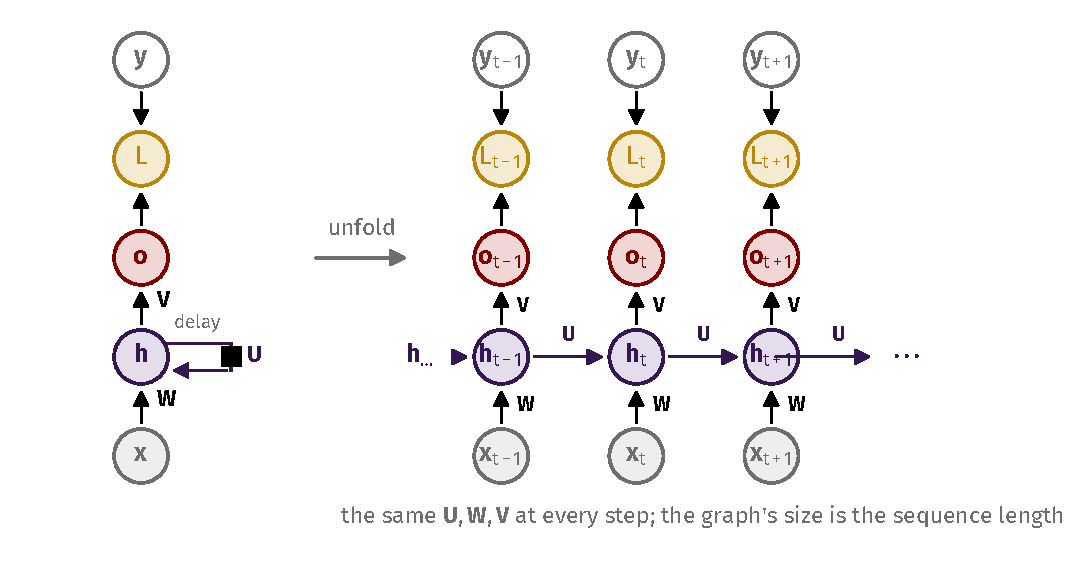
\includegraphics[width=0.78\linewidth]{unfolding}
  \end{center}
  \vspace{-0.7em}
  {\tiny\color{mcMuted}
  Left: the circuit, the black square a delay of one step on the
  recurrent edge $\mathbf{U}$. Right: the unfolded graph, one column per
  step, $\mathbf{W}$, $\mathbf{U}$, $\mathbf{V}$ reused at every column.
  \hfill Layout of Goodfellow et al.\ (2016), Figs.~10.2--10.3.\par}
\end{frame}

\begin{frame}{Three design patterns}
  \begin{center}
    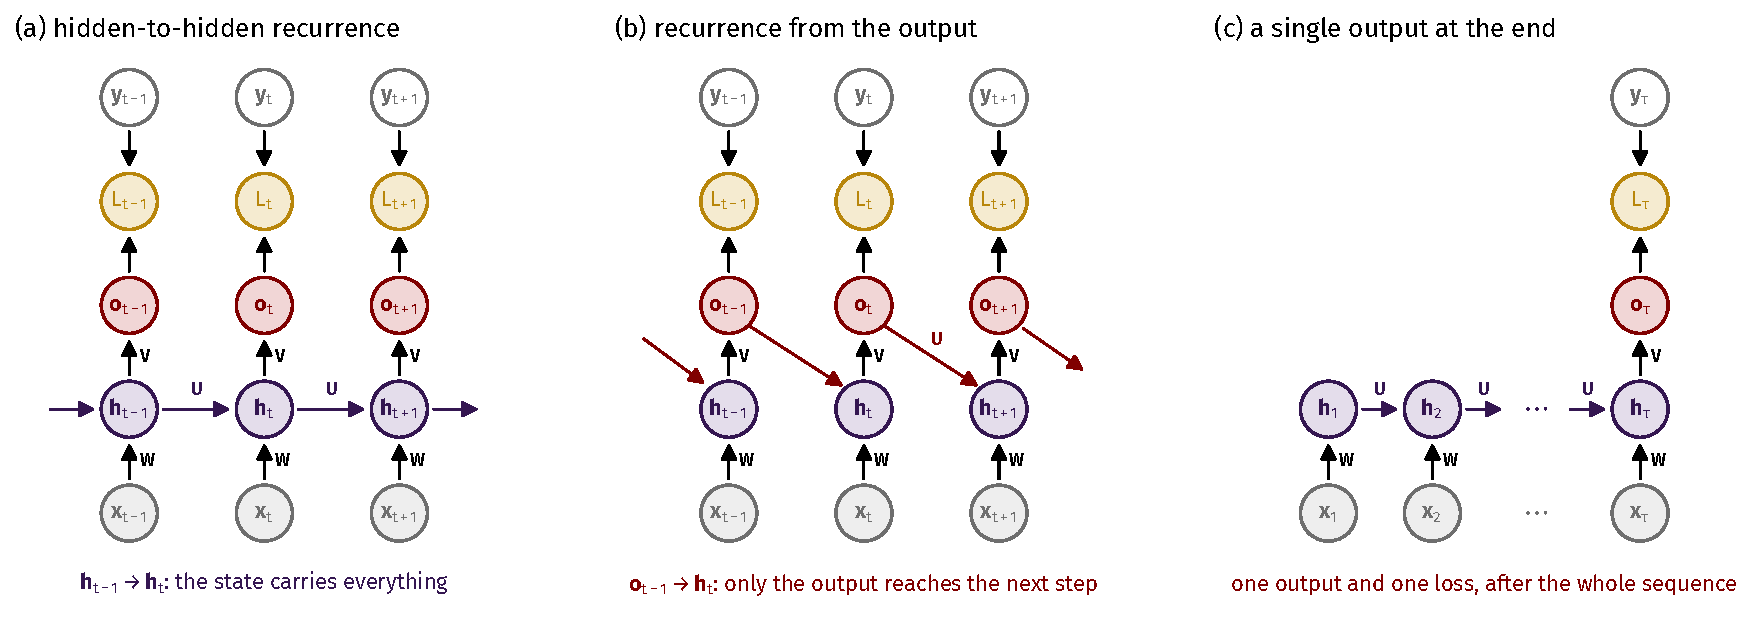
\includegraphics[width=0.92\linewidth]{design_patterns}
  \end{center}
  \vspace{-0.6em}
  {\tiny\color{mcMuted}
  (a) hidden-to-hidden recurrence with an output and a loss at every
  step --- the network of Definition~\ref{th:rnn}, used throughout the
  block. (b) recurrence only from the output: $\mathbf{o}_{t-1}$ is all step
  $t$ learns about the past, so the network is less powerful, but each
  step can be trained on its own (Class 27, teacher forcing). (c) hidden
  recurrence with a single output after the whole sequence: a classifier
  or an encoder.
  \hfill Layouts of Goodfellow et al.\ (2016), Figs.~10.3--10.5.\par}
\end{frame}

\begin{frame}{The loss of a sequence}
  \vspace{0.05em}
  {\footnotesize
  \begin{itemize}\itemsep0.3em
    \item What is the network wrong about? In the running example it
          guessed the next word at every step: \emph{flights} after
          \emph{The}, \ldots, \emph{were} after \emph{canceling}. Each guess
          is a distribution $\hat{\mathbf{y}}_t$ with a right answer $y_t$
    \item So there is a loss at \alert{every step}, the cross-entropy of
          Class 11 --- how little probability the guess gave the truth ---
          and the loss of the sentence is their \alert{sum}:
          \[
            L\big(\{\mathbf{x}_1, \ldots, \mathbf{x}_\tau\}, \{y_1, \ldots, y_\tau\}\big)
            = \sum_{t=1}^{\tau} L_t
            = -\sum_{t=1}^{\tau} \log p_{\mathrm{model}}\big(y_t \mid \mathbf{x}_1, \ldots, \mathbf{x}_t\big),
          \]
          with $p_{\mathrm{model}}(y_t \mid \cdot)$ the entry of $\hat{\mathbf{y}}_t$
          for the true $y_t$
    \item Three sets of weights, $\mathbf{W}$, $\mathbf{U}$, $\mathbf{V}$, each
          used at every step --- so a mistake at step $6$ is partly the
          fault of what $\mathbf{U}$ did at steps $2$ to $5$
  \end{itemize}}
  \srcline{Goodfellow et al.\ (2016), Eqs.~10.12--10.14; Jurafsky \& Martin (2026), \S14.1.2.}
\end{frame}

% =====================================================================
\section{Back-propagation Through Time}
% =====================================================================

\begin{frame}{Why two gradients}
  \vspace{-0.25em}
  {\footnotesize
  \begin{itemize}\itemsep0.2em
    \item The mistake at step $6$: the network said \emph{was}, the
          answer was \emph{were}. Which weights should change, by how
          much? Three matrices, each used six times
    \item Class 11's answer for a feedforward network: walk the graph
          backwards, get the gradient on every \alert{node} from the nodes
          after it, then read the \alert{weights}' gradients off the edges.
          Same here, with two twists
    \item \alert{Twist 1, the nodes.} $\mathbf{h}_3$ has two descendants:
          its own output $\hat{\mathbf{y}}_3$ and the next state $\mathbf{h}_4$.
          The blame reaching it has two parts --- ``your guess at step 3
          was off'' and ``what you handed to step 4 made \emph{its}
          guesses off'' --- so the gradient on the states is a
          \alert{recursion} adding the two, right to left
    \item \alert{Twist 2, the weights.} $\mathbf{U}$ is not one edge but
          six; its gradient is the \alert{sum} of the blame on each use ---
          the state gradient at that step, times what $\mathbf{U}$ was
          multiplying then
    \item Hence two theorems, states then parameters: \alert{back-propagation through time}
  \end{itemize}}
  \srcline{Goodfellow et al.\ (2016), \S10.2.2; Jurafsky \& Martin (2026), \S14.1.2; Class 11.}
\end{frame}
\begin{frame}{The gradient on the states}
  \vspace{-0.45em}
  \begin{thmx}[Back-propagation through time, I]\label{th:bptt}
    \small
    For the network of Definition~\ref{th:rnn} with $L = \sum_t L_t$ and
    $L_t = -\log \hat{y}_t[y_t]$:
    \[
      \nabla_{\mathbf{o}_t}L = \hat{\mathbf{y}}_t - \mathbf{1}_{y_t}, \qquad
      \nabla_{\mathbf{h}_\tau}L = \mathbf{V}^{\top}\nabla_{\mathbf{o}_\tau}L, \qquad
      \nabla_{\mathbf{h}_t}L = \mathbf{U}^{\top}\mathrm{diag}\big(1 - \mathbf{h}_{t+1}^2\big)\,\nabla_{\mathbf{h}_{t+1}}L
                              + \mathbf{V}^{\top}\nabla_{\mathbf{o}_t}L
      \quad (t < \tau).
    \]
  \end{thmx}
  \vspace{-0.1em}
  {\footnotesize
  \begin{itemize}\itemsep0.12em
    \item \focus{1}{Proof. $\partial L/\partial L_t = 1$, and the softmax
          cross-entropy has gradient $\hat{\mathbf{y}}_t - \mathbf{1}_{y_t}$ on
          its scores (Class 11). At the last step $\mathbf{h}_\tau$ has one
          descendant, $\mathbf{o}_\tau = \mathbf{c} + \mathbf{V}\mathbf{h}_\tau$.
          For $t < \tau$ it has two, $\mathbf{o}_t$ and $\mathbf{h}_{t+1}$; the
          chain rule adds a term for each, and
          $\partial\mathbf{h}_{t+1}/\partial\mathbf{h}_t = \mathrm{diag}(1 - \mathbf{h}_{t+1}^2)\,\mathbf{U}$.
          \hfill $\square$}
    \item \focus{2}{A \alert{recursion} that walks the unfolded graph
          right to left, as the forward pass walked it left to right:
          Class 11's back-propagation, on the unfolded graph.}
  \end{itemize}}
  \vspace{-0.3em}
  \srcline{Goodfellow et al.\ (2016), \S10.2.2, Eqs.~10.17--10.21; Jurafsky \& Martin (2026), \S14.1.2; Werbos (1990).}
\end{frame}

\begin{frame}{The two passes, drawn}
  \vspace{-0.3em}
  \begin{center}
    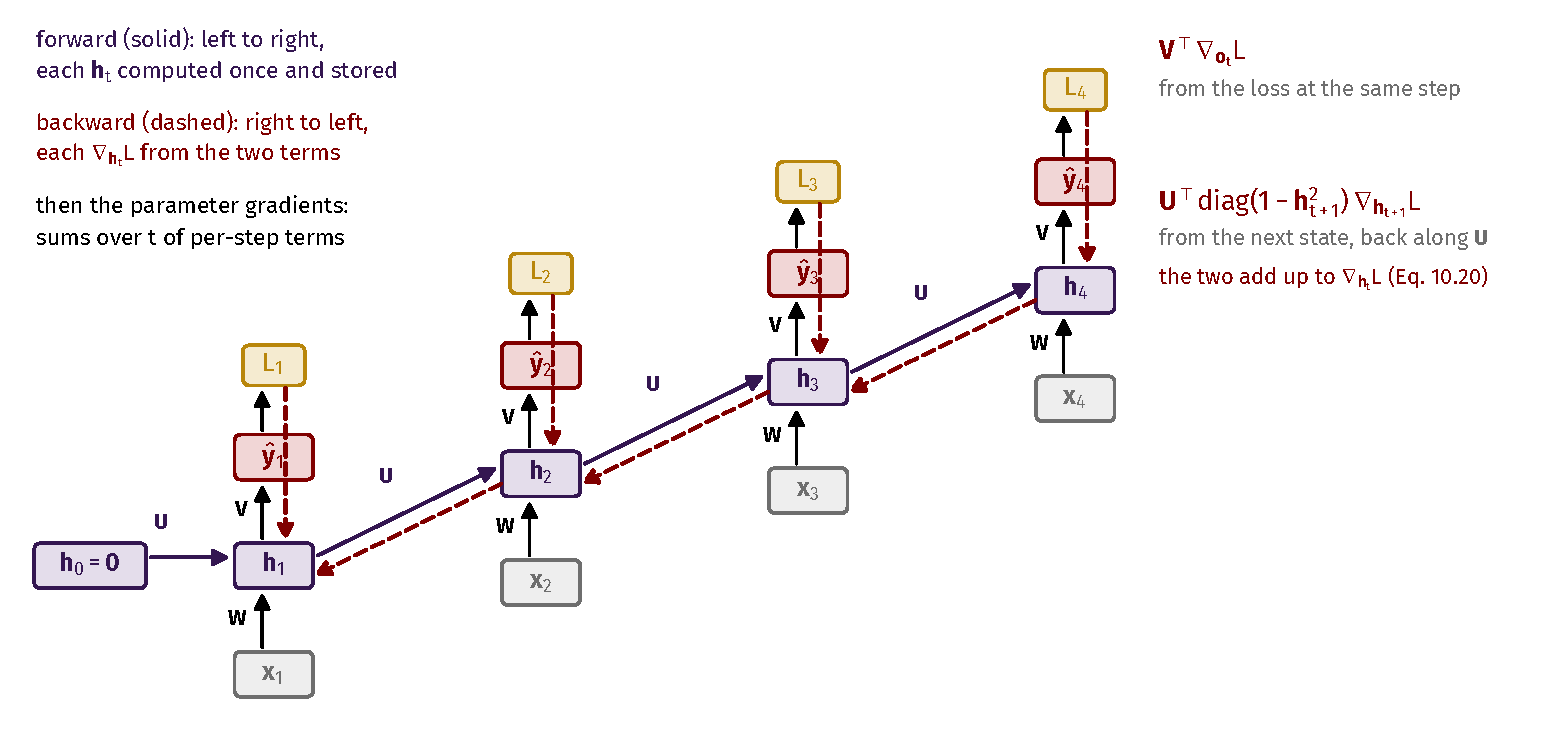
\includegraphics[width=0.80\linewidth]{bptt_flow}
  \end{center}
  \vspace{-0.5em}
  {\tiny\color{mcMuted}
  The unrolled network with both passes. Forward (solid): $\mathbf{h}_t$,
  $\hat{\mathbf{y}}_t$ and $L_t$ from left to right, every $\mathbf{h}_t$ kept.
  Backward (dashed): from right to left, each $\mathbf{h}_t$ receives one
  term from its own loss and one from the state after it, Theorem~\ref{th:bptt}.
  \hfill Layout of Jurafsky \& Martin (2026), Fig.~14.4; Goodfellow et al.\ (2016), Eq.~10.20.\par}
\end{frame}
\begin{frame}{The gradient on the parameters}
  \vspace{-0.45em}
  \begin{thmx}[Back-propagation through time, II]\label{th:bptt2}
    \small
    The gradients on the shared parameters are sums over time:
    \[
      \nabla_{\mathbf{V}}L = \sum_t (\nabla_{\mathbf{o}_t}L)\,\mathbf{h}_t^{\top}, \ \
      \nabla_{\mathbf{U}}L = \sum_t \mathrm{diag}(1 - \mathbf{h}_t^2)(\nabla_{\mathbf{h}_t}L)\,\mathbf{h}_{t-1}^{\top}, \ \
      \nabla_{\mathbf{W}}L = \sum_t \mathrm{diag}(1 - \mathbf{h}_t^2)(\nabla_{\mathbf{h}_t}L)\,\mathbf{x}_t^{\top},
    \]
    $\nabla_{\mathbf{c}}L = \sum_t \nabla_{\mathbf{o}_t}L$,
    $\nabla_{\mathbf{b}}L = \sum_t \mathrm{diag}(1 - \mathbf{h}_t^2)\,\nabla_{\mathbf{h}_t}L$.
  \end{thmx}
  \vspace{-0.1em}
  {\footnotesize
  \begin{itemize}\itemsep0.12em
    \item \focus{1}{Proof. Write $\mathbf{U}_{(t)}$ for the copy of
          $\mathbf{U}$ used at step $t$; a parameter on many edges
          contributes through each, $\nabla_{\mathbf{U}}L = \sum_t \nabla_{\mathbf{U}_{(t)}}L$.
          $\mathbf{a}_t$ is linear in each copy, so the copy's gradient is
          the outer product of $\nabla_{\mathbf{a}_t}L = \mathrm{diag}(1 - \mathbf{h}_t^2)\nabla_{\mathbf{h}_t}L$
          with its input. \hfill $\square$}
    \item \focus{2}{The copies resolve an ambiguity: $\nabla_{\mathbf{U}}$
          in calculus counts every edge, one node's back-propagation
          counts one. No gradient on $\mathbf{x}_t$ is needed.}
  \end{itemize}}
  \vspace{-0.3em}
  \srcline{Goodfellow et al.\ (2016), \S10.2.2, Eqs.~10.22--10.28.}
\end{frame}

\begin{frame}{The theorem, checked: the experiment}
  \vspace{-0.15em}
  {\footnotesize
  \begin{itemize}\itemsep0.28em
    \item \alert{What is being tested.} Theorems~\ref{th:bptt}--\ref{th:bptt2}
          are a procedure for the gradient on every parameter. A wrong one
          --- a transposed matrix, a missing derivative, an off-by-one in
          time --- still runs; it just learns badly
    \item \alert{The setup.} A network of Definition~\ref{th:rnn} with
          $12$ input symbols, $d_h = 8$, $4$ outputs, random weights; a
          batch of $4$ sequences of length $6$, a random target and a
          cross-entropy at every step, so every parameter is in play
    \item \alert{Three ways to the same number.} (1) The theorems, written
          out line by line in NumPy. (2) \alert{Finite differences}: nudge one
          entry by $\pm\epsilon = 10^{-5}$, rerun the forward pass, take
          $(L(\theta + \epsilon) - L(\theta - \epsilon))/2\epsilon$ --- no
          calculus, only the definition of a derivative. (3) The automatic
          differentiation of Class 27's tape: Class 11's rules on the
          unfolded graph
    \item \alert{What agreement would mean.} (1) $=$ (2) to $\approx 10^{-10}$,
          what differencing allows: the theorem is the true derivative.
          (1) $=$ (3) to rounding: it is ordinary back-propagation on the
          unfolded graph
  \end{itemize}}
  \srcline{Goodfellow et al.\ (2016), Eqs.~10.17--10.28; Class 11; Class 27's tape.}
\end{frame}

\begin{frame}{The theorem, checked: the result}
  \begin{center}
    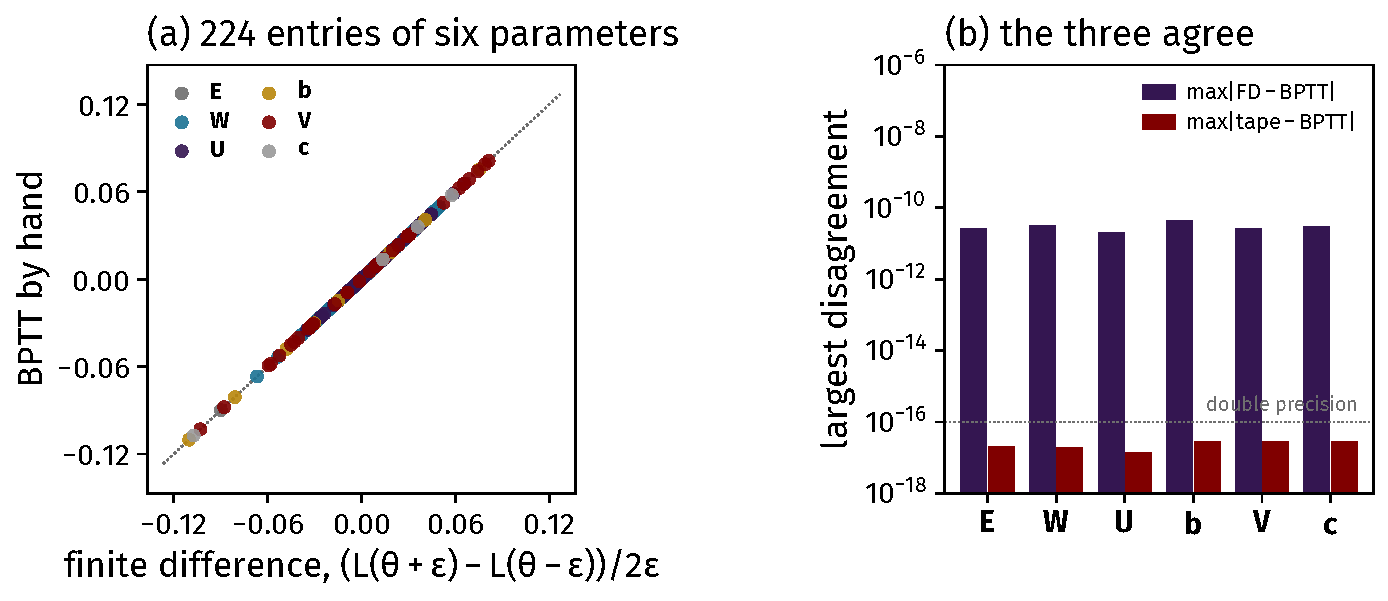
\includegraphics[width=0.78\linewidth]{bptt_check}
  \end{center}
  \vspace{-0.6em}
  {\tiny\color{mcMuted}
  (a) Each of $224$ sampled parameter entries, colour-coded by matrix:
  the hand-written BPTT gradient against the finite-difference estimate.
  Every point lies on the diagonal, for every parameter --- including
  $\mathbf{U}$, whose gradient sums over all six uses. (b) The largest
  disagreement per parameter: about $10^{-11}$ against finite differences,
  which is the differencing error itself, and about $10^{-17}$ against the
  tape, which is double-precision rounding. Both are as small as they can
  be: the theorem is the derivative, and it is ordinary back-propagation.
  \hfill Goodfellow et al.\ (2016), Eqs.~10.17--10.28.\par}
\end{frame}
\begin{frame}{Where the gradient comes from}
  \vspace{-0.45em}
  \begin{corx}[The gradient across a lag is a product]\label{th:product}
    \small
    Iterating the recursion of Theorem~\ref{th:bptt} for a loss at the
    last step only,
    \[
      \nabla_{\mathbf{h}_k}L_\tau
      = \Big( \prod_{s=k+1}^{\tau} \mathbf{U}^{\top}\mathrm{diag}\big(1 - \mathbf{h}_s^2\big) \Big)\,\mathbf{V}^{\top}\nabla_{\mathbf{o}_\tau}L_\tau :
    \]
    the same matrix $\mathbf{U}^{\top}$, times an activation derivative,
    multiplied in once per step of lag.
  \end{corx}
  \vspace{-0.1em}
  {\footnotesize
  \begin{itemize}\itemsep0.12em
    \item \focus{1}{Proof. With $\nabla_{\mathbf{o}_t}L_\tau = \mathbf{0}$ for
          $t < \tau$ the second term of the recursion vanishes; unroll it.
          \hfill $\square$}
    \item \focus{2}{The same product feeds every per-step term of
          Theorem~\ref{th:bptt2}: what reaches $\mathbf{U}$ from step $k$ is
          this, times $\mathbf{h}_{k-1}^{\top}$. So the terms of the sum over
          time are not equal, and a repeated multiplication by one matrix
          is the power iteration of Class 13 --- \alert{Class 28 starts
          here}.}
  \end{itemize}}
  \vspace{-0.3em}
  \srcline{Goodfellow et al.\ (2016), Eq.~10.21 iterated, \S10.7; Class 13; Class 28.}
\end{frame}

\begin{frame}{The terms of the sum: the experiment}
  \vspace{-0.15em}
  {\footnotesize
  \begin{itemize}\itemsep0.28em
    \item \alert{What is being measured.} Theorem~\ref{th:bptt2} makes
          $\nabla_{\mathbf{U}}L$ a sum of one term per step;
          Corollary~\ref{th:product} says the term at step $t$ carries a
          product of $\tau - t$ Jacobians. So which steps does the gradient
          come from?
    \item \alert{The setup.} The running example made abstract: sequences
          of length $16$ whose \alert{first} symbol must be recalled at the
          \alert{last} step, fillers between --- a dependency $15$ steps long;
          one loss, at the end; $d_h = 16$, at random initialisation and
          after $1{,}500$ training steps (accuracy $1.00$)
    \item \alert{Two quantities off the backward recursion.} (a)
          $\|\nabla_{\mathbf{h}_t}L\|$ for $t = 1 \ldots 16$; (b) the norm of the
          per-step term of $\nabla_{\mathbf{U}}L$,
          $\|\mathrm{diag}(1 - \mathbf{h}_t^2)(\nabla_{\mathbf{h}_t}L)\,\mathbf{h}_{t-1}^{\top}\|$;
          both relative to the last step, so the plot shows shape, not scale
    \item \alert{What to expect.} At initialisation, $\|\mathbf{U}\| \approx 1$
          and $\tanh$ derivatives below one: the product shrinks with every
          step of lag, a curve falling right to left. After training the
          early steps should matter more --- whether the curve becomes flat
          is the question
  \end{itemize}}
  \srcline{Goodfellow et al.\ (2016), Eqs.~10.20, 10.26, \S10.7.}
\end{frame}

\begin{frame}{The terms of the sum: the result}
  \begin{center}
    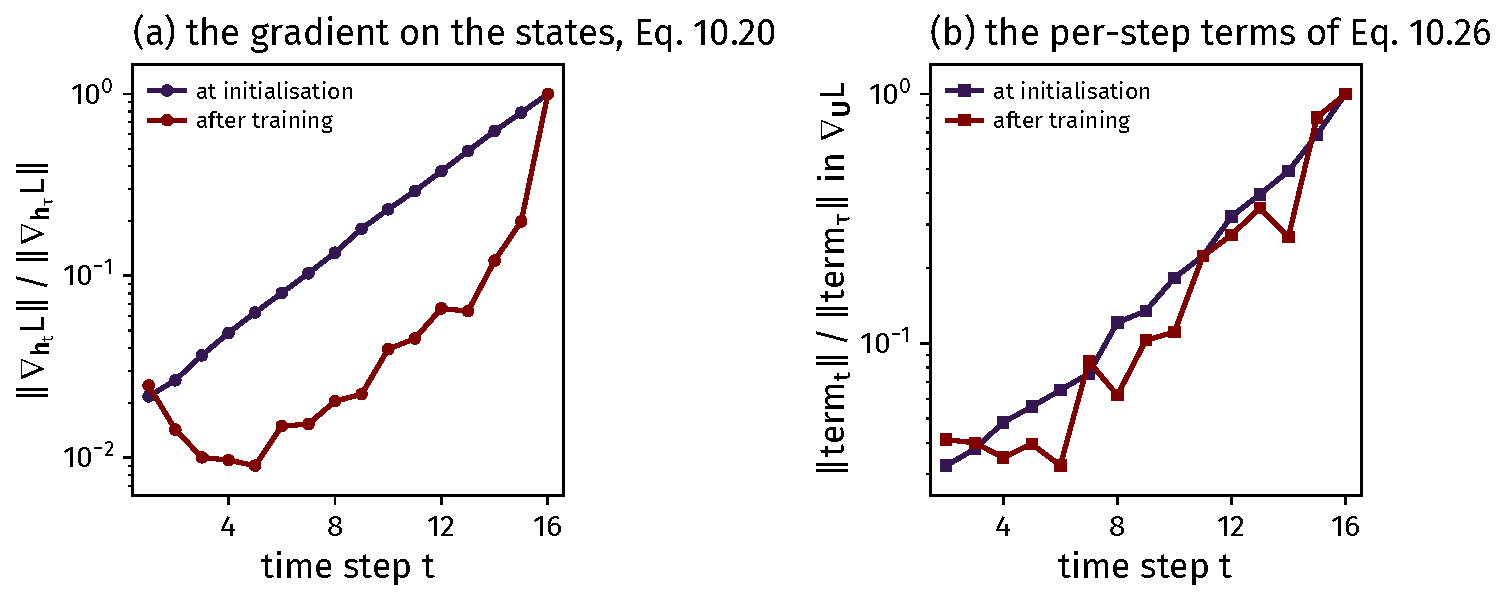
\includegraphics[width=0.80\linewidth]{time_contributions}
  \end{center}
  \vspace{-0.6em}
  {\tiny\color{mcMuted}
  (a) At initialisation (indigo) the gradient on the states falls
  steadily from the last step back to the first: by a factor of about
  $40$ over $15$ steps, one shrinking factor per step, as the corollary
  predicts. After training (maroon) the curve is reshaped --- it dips in
  the middle and rises again towards the first step, where the symbol
  the network learned to carry was read --- but it is not flat. (b) The
  per-step terms of $\nabla_{\mathbf{U}}L$ follow the same shape: the sum
  over time is dominated by the last few steps, before and after
  training. This is the expected outcome, and it is the problem Class 28
  is about.
  \hfill Goodfellow et al.\ (2016), Eqs.~10.20, 10.26, \S10.7.\par}
\end{frame}

% =====================================================================
\section{The Cost of Time}
% =====================================================================

\begin{frame}{Two passes, sequential}
  \vspace{-0.45em}
  \begin{propx}[Cost of the unrolled graph]\label{th:cost}
    \small
    For a sequence of length $\tau$, the forward pass and the backward
    pass each take $O(\tau)$ time, the forward pass cannot be
    parallelised across steps, and the backward pass needs every
    $\mathbf{h}_t$ from the forward pass, so the memory is $O(\tau)$ as well.
  \end{propx}
  \vspace{-0.1em}
  {\footnotesize
  \begin{itemize}\itemsep0.12em
    \item \focus{1}{Proof. One step of Definition~\ref{th:rnn} costs a
          fixed amount and needs $\mathbf{h}_{t-1}$, so $\tau$ steps cost
          $\tau$ times that, in order. Theorem~\ref{th:bptt2} multiplies by
          $\mathbf{h}_t$, $\mathbf{h}_{t-1}$ and $1 - \mathbf{h}_t^2$ at every $t$,
          so all of them must be kept. \hfill $\square$}
    \item \focus{2}{Contrast convolution, whose positions run at once.
          Depth in time is paid serially --- one reason the transformer
          (Classes 30--31) gives the recurrence up.}
    \item \focus{3}{No specialised algorithm is needed: unroll the
          network for the given input, and ordinary back-propagation on
          that graph is BPTT. Class 27's tape does exactly this.}
  \end{itemize}}
  \vspace{-0.3em}
  \srcline{Goodfellow et al.\ (2016), \S10.2; Jurafsky \& Martin (2026), \S14.1.2.}
\end{frame}

\begin{frame}{The cost, measured}
  \begin{center}
    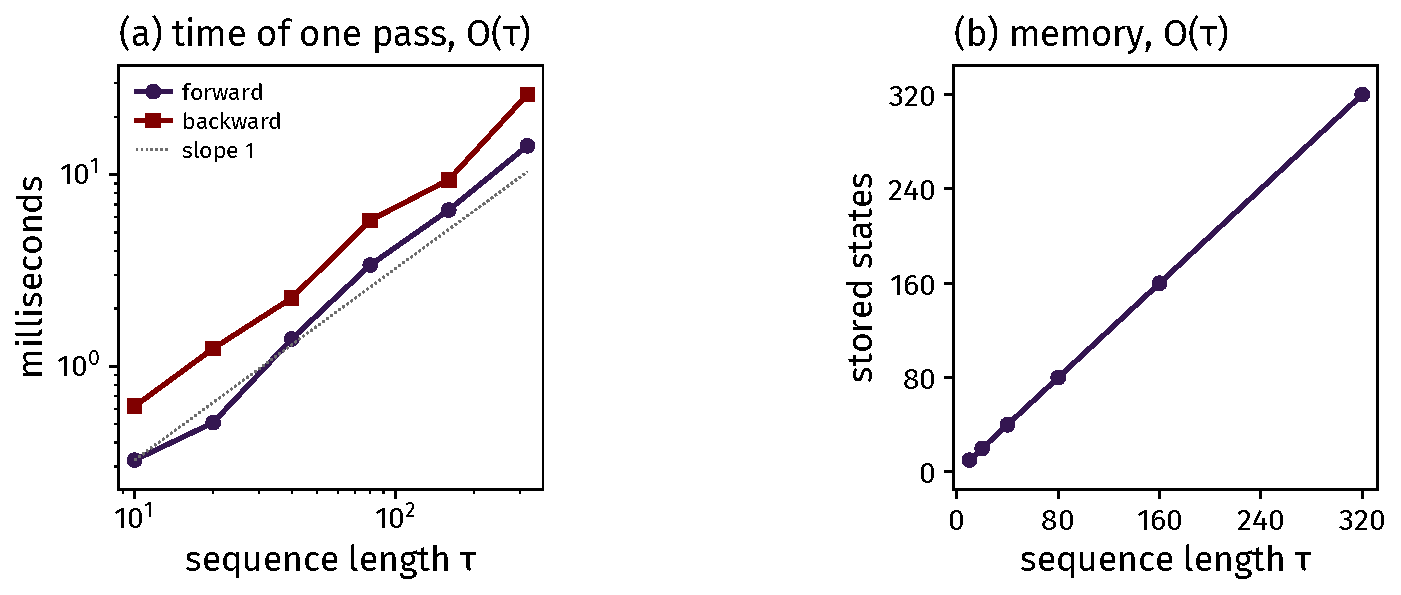
\includegraphics[width=0.84\linewidth]{cost}
  \end{center}
  \vspace{-0.6em}
  {\tiny\color{mcMuted}
  The network of Definition~\ref{th:rnn} with $d_h = 32$ on a batch of
  $16$, on the tape of Class 27. (a) wall-clock time of one forward and
  one backward pass against the sequence length, on log axes with a
  slope-one reference: both are linear in $\tau$. (b) the number of
  hidden states the backward pass reads: one per step.
  \hfill Goodfellow et al.\ (2016), \S10.2.\par}
\end{frame}

\begin{frame}{Truncation}
  \vspace{0.05em}
  {\footnotesize
  \begin{itemize}\itemsep0.3em
    \item For long inputs --- speech, character-level text, streaming
          input --- unrolling the whole sequence may not be feasible:
          the graph, and the memory of Proposition~\ref{th:cost}, grow
          with it
    \item The practice is to unroll the input into manageable
          \alert{fixed-length segments} and treat each segment as a
          distinct training item; the hidden state still carries forward
          across the cut, so the forward pass is the same as before
    \item What changes is the backward pass: it stops at the segment
          boundary, so the gradient at a step only reaches back as far as
          the segment allows; how far a dependency can reach in the
          forward pass and how far it can be trained are no longer the
          same distance
  \end{itemize}}
  \srcline{Jurafsky \& Martin (2026), \S14.1.2; Williams \& Peng (1990).}
\end{frame}

% =====================================================================
\section{Both Directions}
% =====================================================================

\begin{frame}{Why a second direction}
  \vspace{0.05em}
  {\footnotesize
  \begin{itemize}\itemsep0.25em
    \item Everything so far reads \alert{left to right}: $\mathbf{h}_t$
          summarises $\mathbf{x}_1 \ldots \mathbf{x}_t$ and knows nothing after.
          For predicting the next word that is right: the future is what
          is being predicted
    \item But many tasks have the \alert{whole input in hand}, and the
          answer at $t$ depends on what follows. Tag \emph{back} in
          ``\emph{back} the bill'' (verb) against ``\emph{back} and neck
          ached'' (noun): at $t = 1$ a left-to-right reader has seen only
          \emph{back}
    \item Speech likewise: which phoneme a sound is depends on the next
          few, by co-articulation; which word, on the next few words
    \item The fix is not a bigger window but a \alert{second chain}, read
          from the end, whose state at $t$ summarises $\mathbf{x}_t \ldots \mathbf{x}_n$;
          side by side, the two states let the output at $t$ see both sides
  \end{itemize}}
  \srcline{Goodfellow et al.\ (2016), \S10.3; Jurafsky \& Martin (2026), \S14.4.2; Class 29.}
\end{frame}
\begin{frame}{Reading the sequence both ways}
  \vspace{-0.45em}
  \begin{defx}[Bidirectional RNN]\label{th:bi}
    \small
    Two independent recurrent networks, one read from the start and one
    from the end, their states concatenated at each step:
    \[
      \mathbf{h}^{f}_t = \mathrm{RNN}_{\mathrm{forward}}(\mathbf{x}_1, \ldots, \mathbf{x}_t), \qquad
      \mathbf{h}^{b}_t = \mathrm{RNN}_{\mathrm{backward}}(\mathbf{x}_t, \ldots, \mathbf{x}_n), \qquad
      \mathbf{h}_t = [\mathbf{h}^{f}_t ; \mathbf{h}^{b}_t],
    \]
    and the output $\mathbf{o}_t$ computed from $\mathbf{h}_t$.
  \end{defx}
  \vspace{-0.1em}
  {\footnotesize
  \begin{itemize}\itemsep0.16em
    \item Every network so far is \alert{causal}: $\mathbf{h}_t$ knows
          nothing after $\mathbf{x}_t$. Many predictions need the future
          too --- a phoneme depends on the next few, a word on the next words
    \item $\mathbf{h}^{b}_t$ is the ordinary state of a network run on the
          reversed input; Goodfellow's $\mathbf{g}^{(t)}$ is Jurafsky's
          $\mathbf{h}^{b}_t$. Sum or product also combine them; four chains
          do the same on a 2-D grid
  \end{itemize}}
  \vspace{-0.3em}
  \srcline{Jurafsky \& Martin (2026), \S14.4.2, Eqs.~14.16--14.18; Goodfellow et al.\ (2016), \S10.3; Schuster \& Paliwal (1997).}
\end{frame}

\begin{frame}{What the second direction changes}
  \vspace{-0.45em}
  \begin{propx}[The bidirectional output sees the whole input]\label{th:bidep}
    \small
    In a bidirectional RNN the output $\mathbf{o}_t$ is a function of
    $\mathbf{x}_1, \ldots, \mathbf{x}_n$ for every $t$, most sensitive to the
    inputs near $t$ but with no fixed window; the cost is twice one
    direction; and the network is not causal, so it needs the whole input
    before any output and cannot generate a sequence step by step.
  \end{propx}
  \vspace{-0.1em}
  {\footnotesize
  \begin{itemize}\itemsep0.12em
    \item \focus{1}{Proof. $\mathbf{h}^{f}_t$ depends on $\mathbf{x}_{\leq t}$ and
          $\mathbf{h}^{b}_t$ on $\mathbf{x}_{\geq t}$ by Proposition~\ref{th:unfold}
          applied to each chain; $\mathbf{o}_t$ reads both. Each chain is
          one forward pass of Proposition~\ref{th:cost}. \hfill $\square$}
    \item \focus{2}{Training is unchanged: unroll both chains and
          back-propagate; the backward chain's BPTT runs left to right.}
    \item \focus{3}{Used for labelling and classification (Class 29)
          and the encoder of Class 27; not for language modelling or
          decoding, which emit the next token from the past alone.}
  \end{itemize}}
  \vspace{-0.3em}
  \srcline{Goodfellow et al.\ (2016), \S10.3; Jurafsky \& Martin (2026), \S14.4.2.}
\end{frame}

\begin{frame}{Both directions, drawn}
  \vspace{-0.3em}
  \begin{center}
    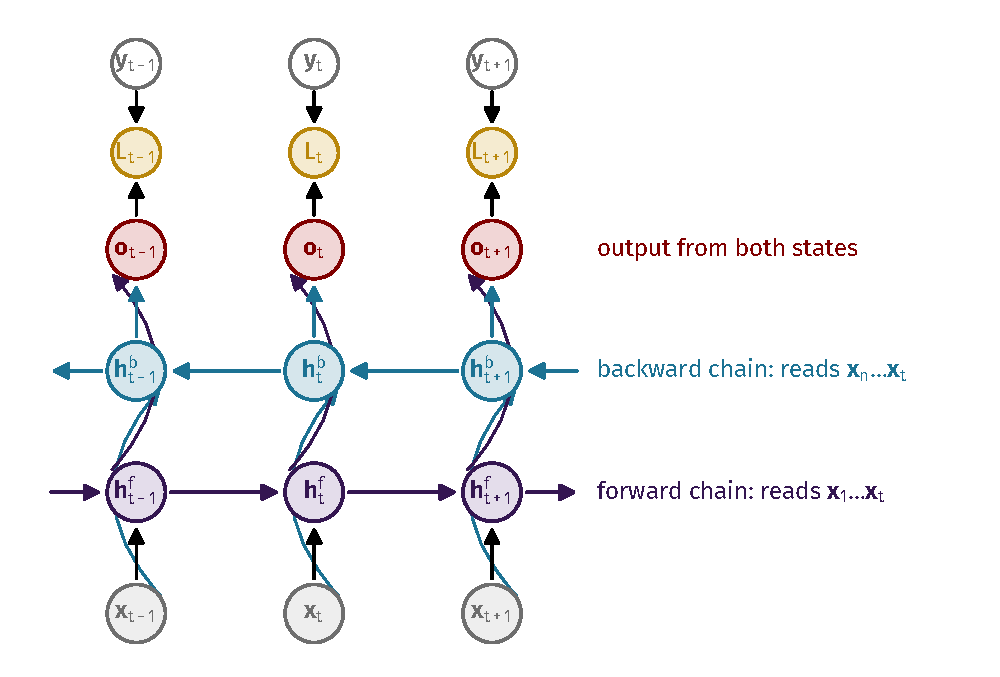
\includegraphics[width=0.56\linewidth]{bidirectional_goodfellow}
  \end{center}
  \vspace{-0.5em}
  {\tiny\color{mcMuted}
  Goodfellow's drawing, in Jurafsky's names: the forward chain
  $\mathbf{h}^f$ (Goodfellow's $h$) moves left to right, the backward chain
  $\mathbf{h}^b$ (his $g$) right to left; each input $\mathbf{x}_t$ feeds
  both, and the output $\mathbf{o}_t$ reads both states, so it depends on
  the past and the future but is most sensitive to the inputs near $t$.
  \hfill Layout of Goodfellow et al.\ (2016), Fig.~10.11.\par}
\end{frame}

\begin{frame}{Both directions, as two networks}
  \vspace{-0.3em}
  \begin{center}
    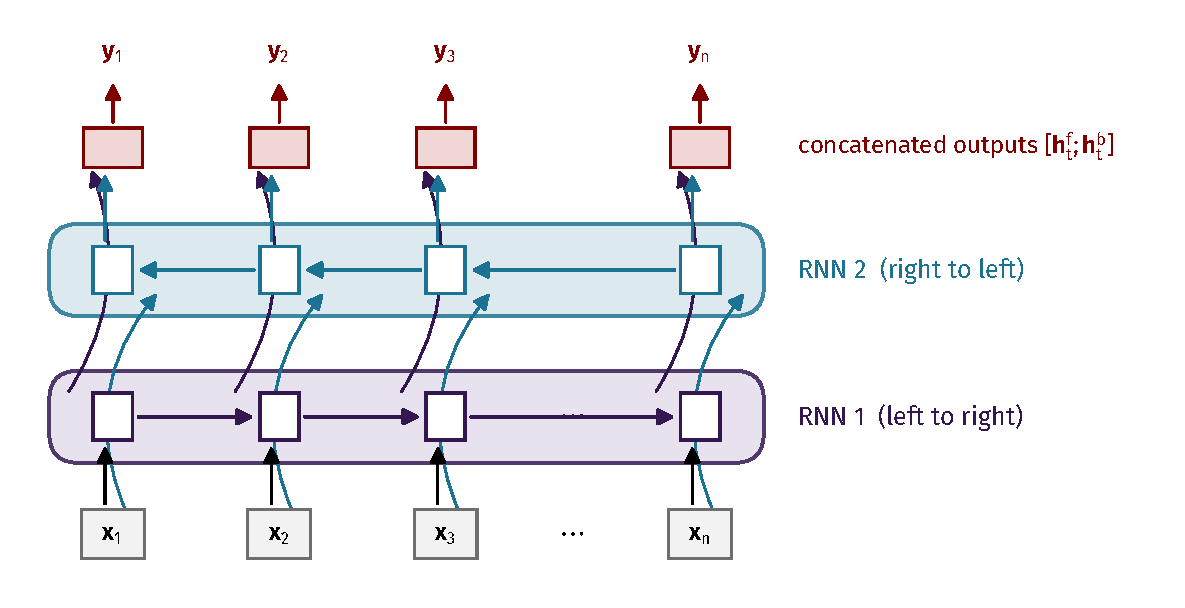
\includegraphics[width=0.74\linewidth]{bidirectional_jurafsky}
  \end{center}
  \vspace{-0.5em}
  {\tiny\color{mcMuted}
  Jurafsky's drawing: two separate recurrent networks, RNN 1 trained
  left to right and RNN 2 right to left, each reading every input; at each
  step their two states are concatenated, $[\mathbf{h}^f_t ; \mathbf{h}^b_t]$,
  and that vector is the representation of position $t$ from which the
  output $\mathbf{y}_t$ is computed. Nothing inside either network changes;
  only the read-out sees both.
  \hfill Layout of Jurafsky \& Martin (2026), Fig.~14.11.\par}
\end{frame}

\begin{frame}{Both directions, measured}
  \begin{center}
    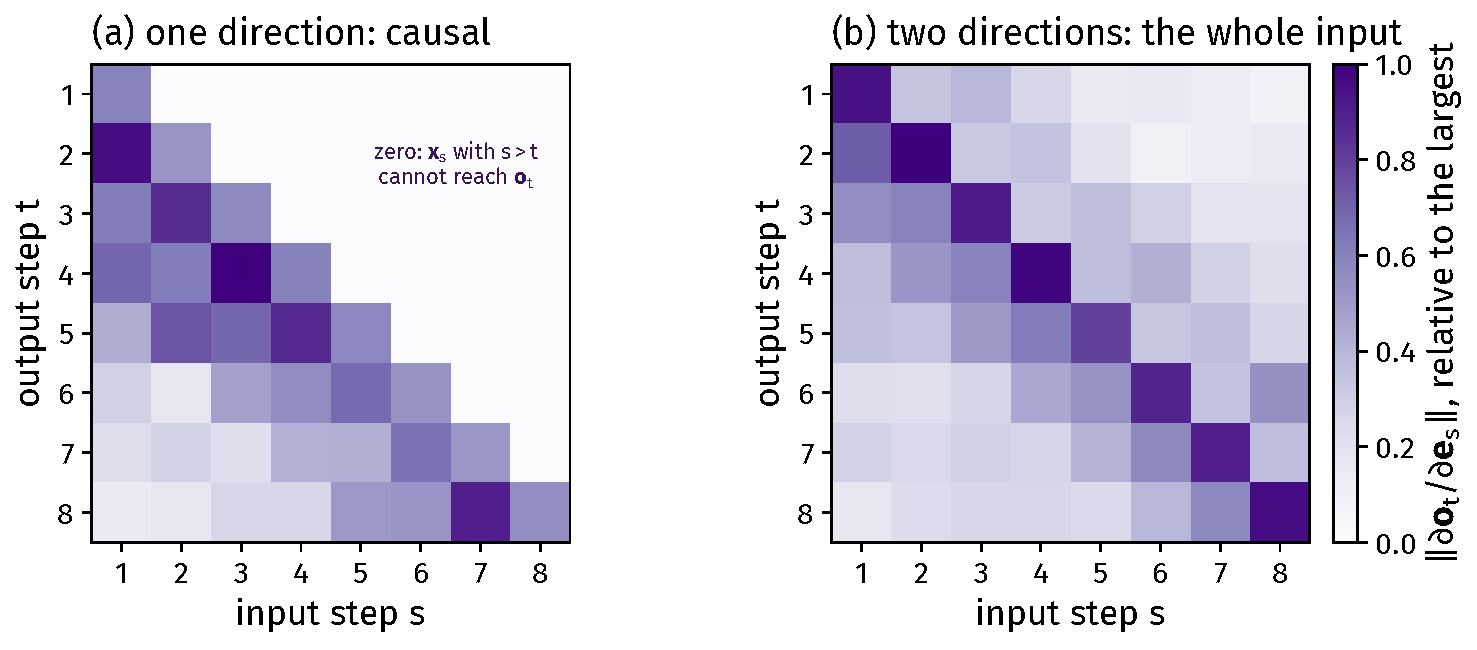
\includegraphics[width=0.80\linewidth]{influence_maps}
  \end{center}
  \vspace{-0.6em}
  {\tiny\color{mcMuted}
  Each square is one number read off the tape: how much the output at
  step $t$ (row) changes when the input at step $s$ (column) changes,
  $\|\partial\mathbf{o}_t/\partial\mathbf{e}_s\|$, for a random length-$8$
  input at initialisation, relative to the largest entry. (a) A
  one-directional network: everything above the diagonal is exactly
  zero --- an input after $t$ cannot reach $\mathbf{o}_t$ --- and the
  influence fades with distance below it. (b) A bidirectional network:
  every square is nonzero, the diagonal is darkest, and the influence
  fades in both directions from it: the whole input, most sensitive near $t$.
  \hfill Goodfellow et al.\ (2016), \S10.3.\par}
\end{frame}

% =====================================================================
\section{Putting It Together}
% =====================================================================

\begin{frame}{The block ahead, revisited}
  \vspace{0.2em}
  {\scriptsize
  \renewcommand{\arraystretch}{1.36}
  \begin{tabular}{@{}l@{\hspace{1.0em}}l@{\hspace{1.0em}}l@{}}
    \textbf{Class} & \textbf{takes from today} & \textbf{adds}\\
    27 --- encoder--decoder & the cell as a black box; unfolding; BPTT & two chains, a context, attention\\
    28 --- LSTM and gates & Corollary~\ref{th:product}: the product of Jacobians & why it vanishes, a path that does not\\
    29 --- NLP tasks & Definition~\ref{th:bi}; the three design patterns & what to read out, where to pay the loss\\
    30--31 --- transformers & Proposition~\ref{th:cost}: time is paid serially & attention without recurrence\\
  \end{tabular}}
  \vspace{0.6em}

  \begin{redhighlight}
    Unfold, and a recurrent network is a deep feedforward network with
    its weights tied across layers. Everything about training it follows
    from that one picture.
  \end{redhighlight}
\end{frame}

\begin{frame}{Takeaways}
  \vspace{-0.1em}
  {\scriptsize
  \begin{enumerate}\itemsep0.24em
    \item A sequence has any length, an order, and dependencies that
          reach; a window cannot follow them, a state carried step by step
          can --- the same weight sharing as convolution, across time
          instead of space
    \item A simple recurrent network is one feedforward step with two
          inputs, the current $\mathbf{x}_t$ and the previous $\mathbf{h}_{t-1}$,
          applied with the same $\mathbf{U}, \mathbf{W}, \mathbf{V}$ at every
          step (Definition~\ref{th:rnn}); unfolded, it is a DAG whose size
          is the sequence length and whose parameter count is not
          (Proposition~\ref{th:unfold})
    \item Back-propagation through time is back-propagation on that
          graph: a backward recursion over the states, then sums over time
          for the shared parameters (Theorems~\ref{th:bptt}--\ref{th:bptt2}),
          verified here to $10^{-11}$ against finite differences
    \item Across a lag the gradient is a product of one matrix and one
          derivative per step (Corollary~\ref{th:product}); measured, the
          recent steps dominate the sum
    \item Both passes are $O(\tau)$ in time and memory and serial in time
          (Proposition~\ref{th:cost}); training on segments of $k$ steps
          stops the backward pass at the cut
    \item A bidirectional network runs a second chain from the end; its
          output at $t$ sees the whole input and it is no longer causal
          (Definition~\ref{th:bi}, Proposition~\ref{th:bidep})
  \end{enumerate}}
  \vspace{-0.2em}
  \bridge{Class 27: two of these networks, one reading and one writing --- the encoder--decoder.}
\end{frame}

\begin{frame}[allowframebreaks]{References}
  {\scriptsize
  \begin{itemize}\itemsep0.3em
    \item Jurafsky, D. \& Martin, J. H. (2026). \emph{Speech and Language
          Processing}, 3rd ed.\ draft, August 2026. Ch.~14, \S14.1, \S14.4.2.
    \item Goodfellow, I., Bengio, Y. \& Courville, A. (2016). \emph{Deep
          Learning}. MIT Press. \S10.1--10.2.2, \S10.3.
    \item Elman, J. L. (1990). Finding structure in time. \emph{Cognitive
          Science}, 14, 179--211.
    \item Rumelhart, D. E., Hinton, G. E. \& Williams, R. J. (1986). Learning
          representations by back-propagating errors. \emph{Nature}, 323,
          533--536.
    \item Werbos, P. J. (1990). Backpropagation through time: what it does
          and how to do it. \emph{Proceedings of the IEEE}, 78, 1550--1560.
    \item Williams, R. J. \& Peng, J. (1990). An efficient gradient-based
          algorithm for on-line training of recurrent network trajectories.
          \emph{Neural Computation}, 2, 490--501.
    \item Schuster, M. \& Paliwal, K. K. (1997). Bidirectional recurrent
          neural networks. \emph{IEEE Trans.\ Signal Processing}, 45,
          2673--2681.
    \item Siegelmann, H. T. \& Sontag, E. D. (1995). On the computational
          power of neural nets. \emph{Journal of Computer and System
          Sciences}, 50, 132--150.
    \item Graves, A. (2012). \emph{Supervised Sequence Labelling with
          Recurrent Neural Networks}. Springer.
  \end{itemize}}
\end{frame}

\begin{frame}[standout]
  Questions?
\end{frame}

\end{document}
